\documentclass{article}
\usepackage{graphicx}
\graphicspath{{./images/}}
\usepackage{float}
\usepackage{caption}
\usepackage{subcaption}
\usepackage{parskip}
\usepackage{amsmath}
\usepackage[margin=15mm]{geometry}
\usepackage[titletoc,toc,title]{appendix}
\usepackage{hyperref}

\title{CS3210 Lab 2}
\author{Leow Li Yong}
\date{17 February 2025}

\begin{document}
% \sffamily
\captionsetup{justification=centering}
\maketitle

\section{Code Description}
The program take in 2 integers as inputs. First input \textit{size} is used to generate 2 square matrices of size \textit{size} x \textit{size}. The matrices are then multiplied together to a new matrix and the time taken to do so is printed to stdout. OpenMP was used to parallelize the matrix multiplication algorithm and the number of threads used was set with the second integer input.  

\section{Comparing Processors}
A bash script executed the program on two machines: one with an Intel i7-7700 (4 physical, 8 logical cores) and another with an Intel XS-4114 (10 physical, 20 logical cores). Programs were run via Slurm to ensure exclusive node access. Thread counts ranged from 1 to 8192 (doubled iteratively), with matrix size fixed at 1500 to ensure $\geq$1s execution. Each configuration was run three times, with \texttt{perf} recording cycles, instructions, and floating-point operations. Data was parsed into CSV format, and the results are shown in Figure~\ref{fig:graphsColWise}.

\begin{figure}[H]
	\centering
	\begin{subfigure}{0.5\textwidth}
		\centering
		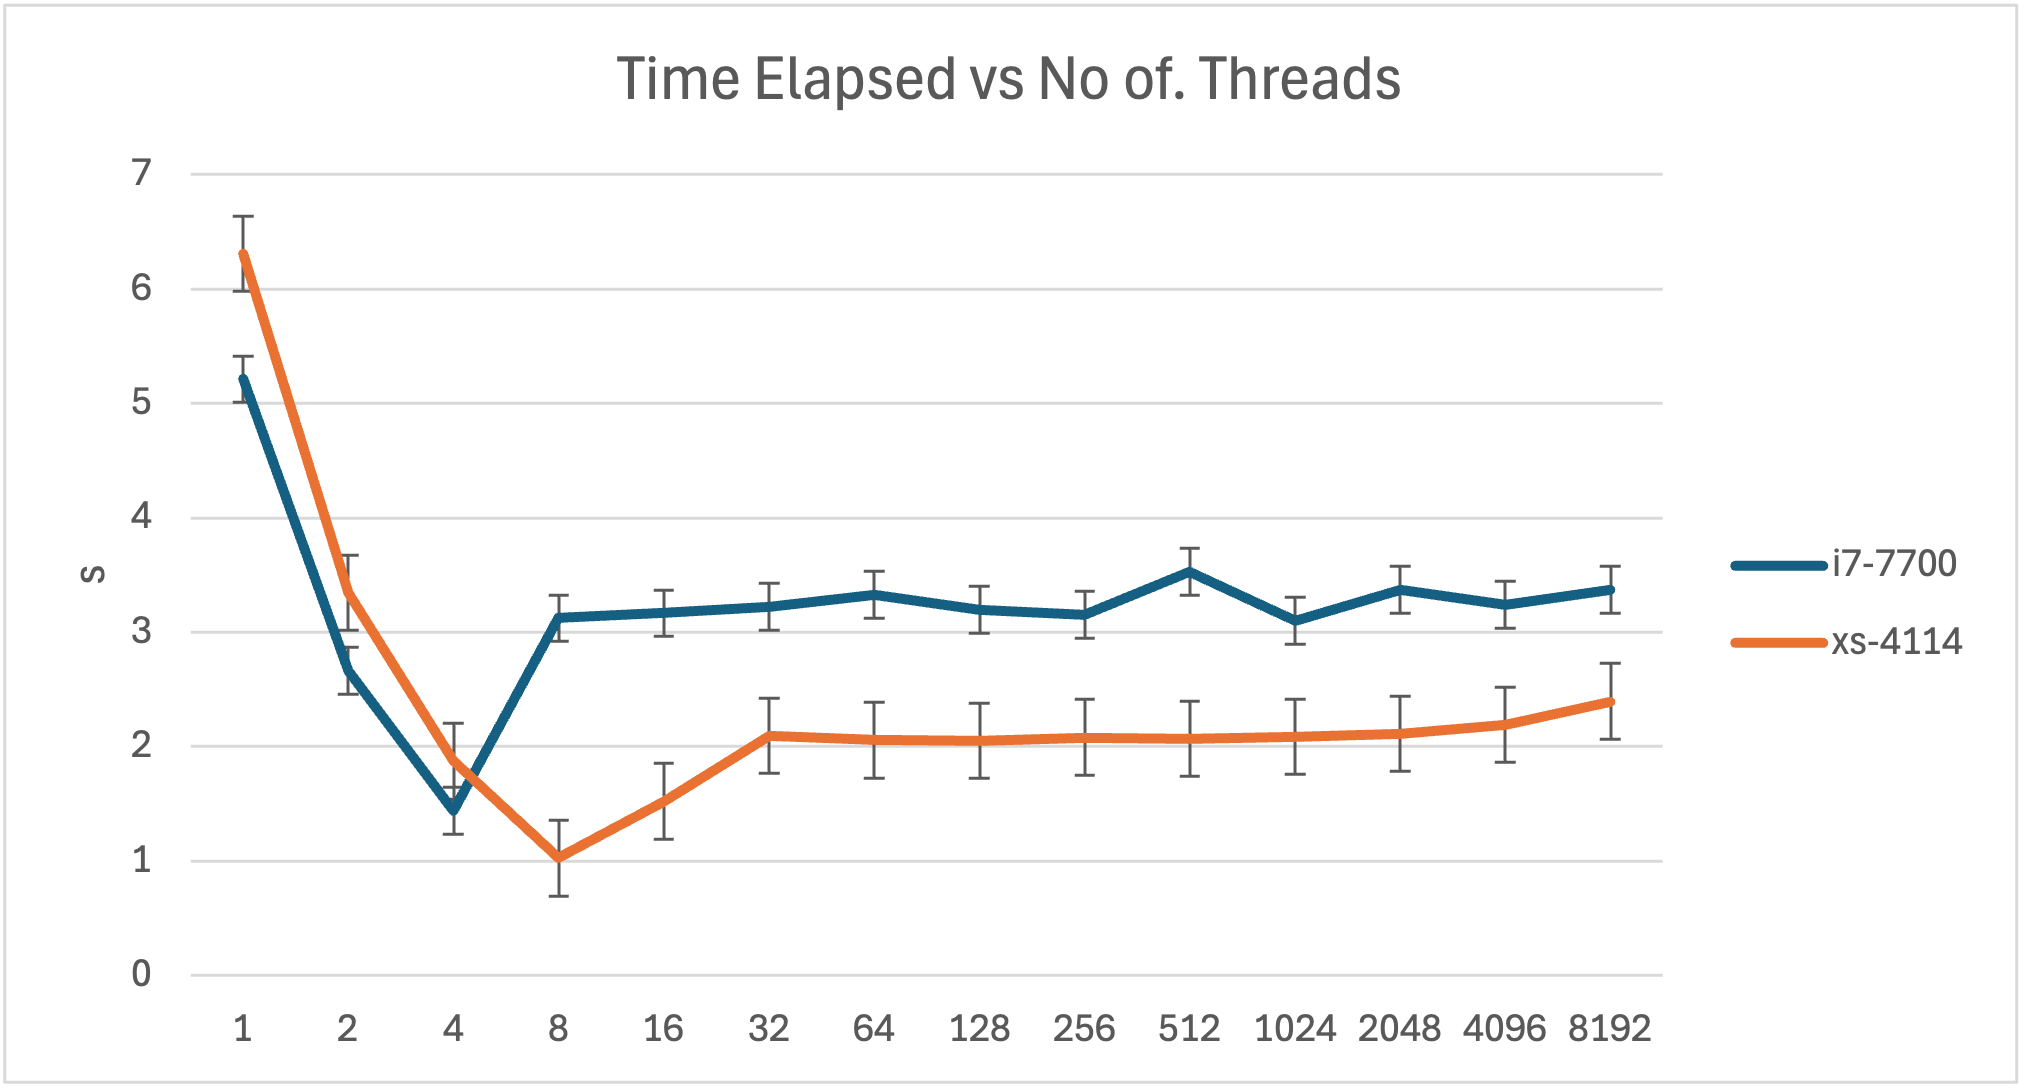
\includegraphics[width=0.8\linewidth]{timeElapsed.png}
		\subcaption{Time elapsed vs. threads}
		\label{fig:timeGraph}
	\end{subfigure}%
	\begin{subfigure}{0.5\textwidth}
		\centering
		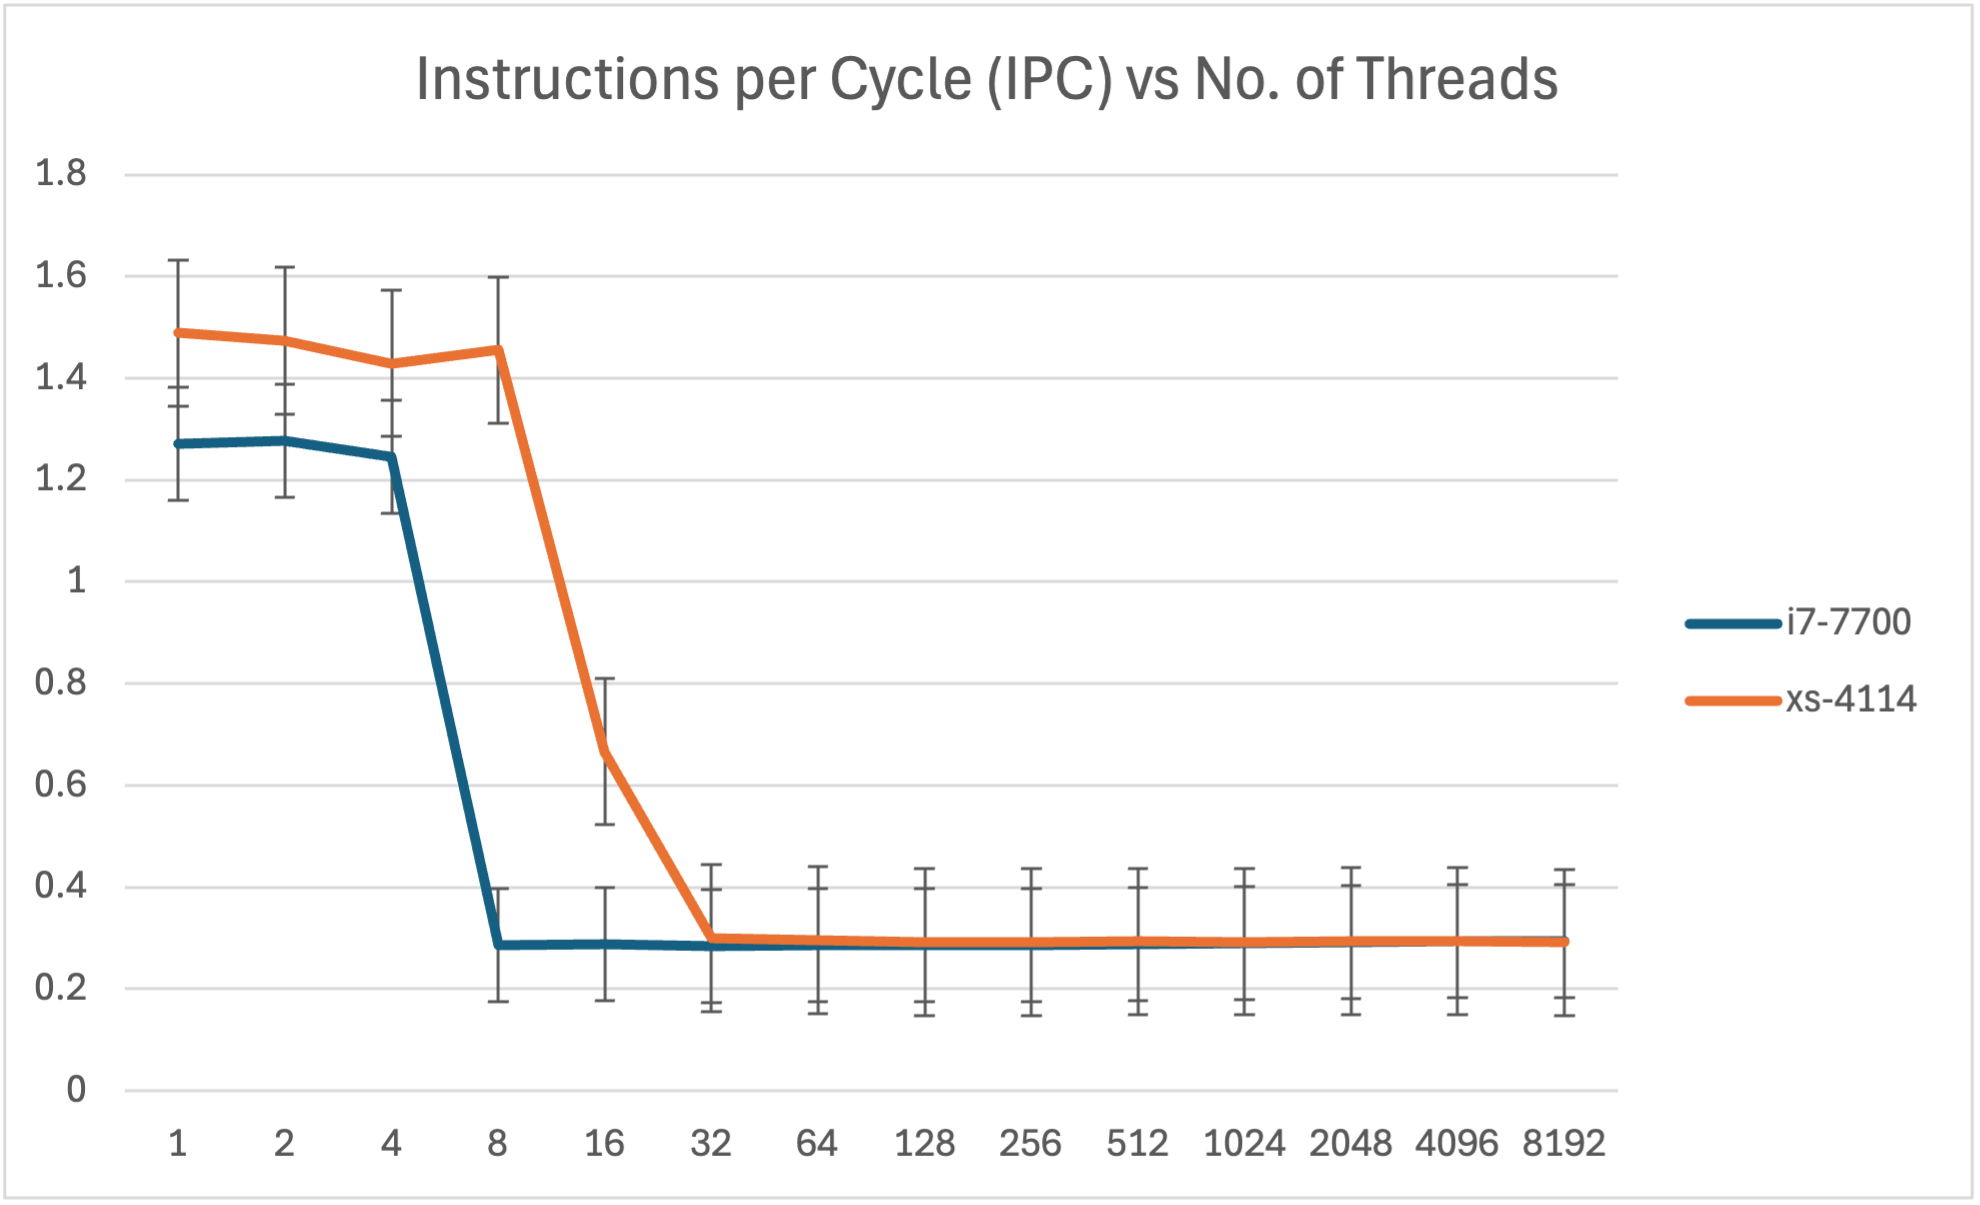
\includegraphics[width=0.8\linewidth]{ipc.png}
		\subcaption{IPC vs. threads}
		\label{fig:ipcGraph}
	\end{subfigure}%
	\newline
	\begin{subfigure}{0.5\textwidth}
		\centering
		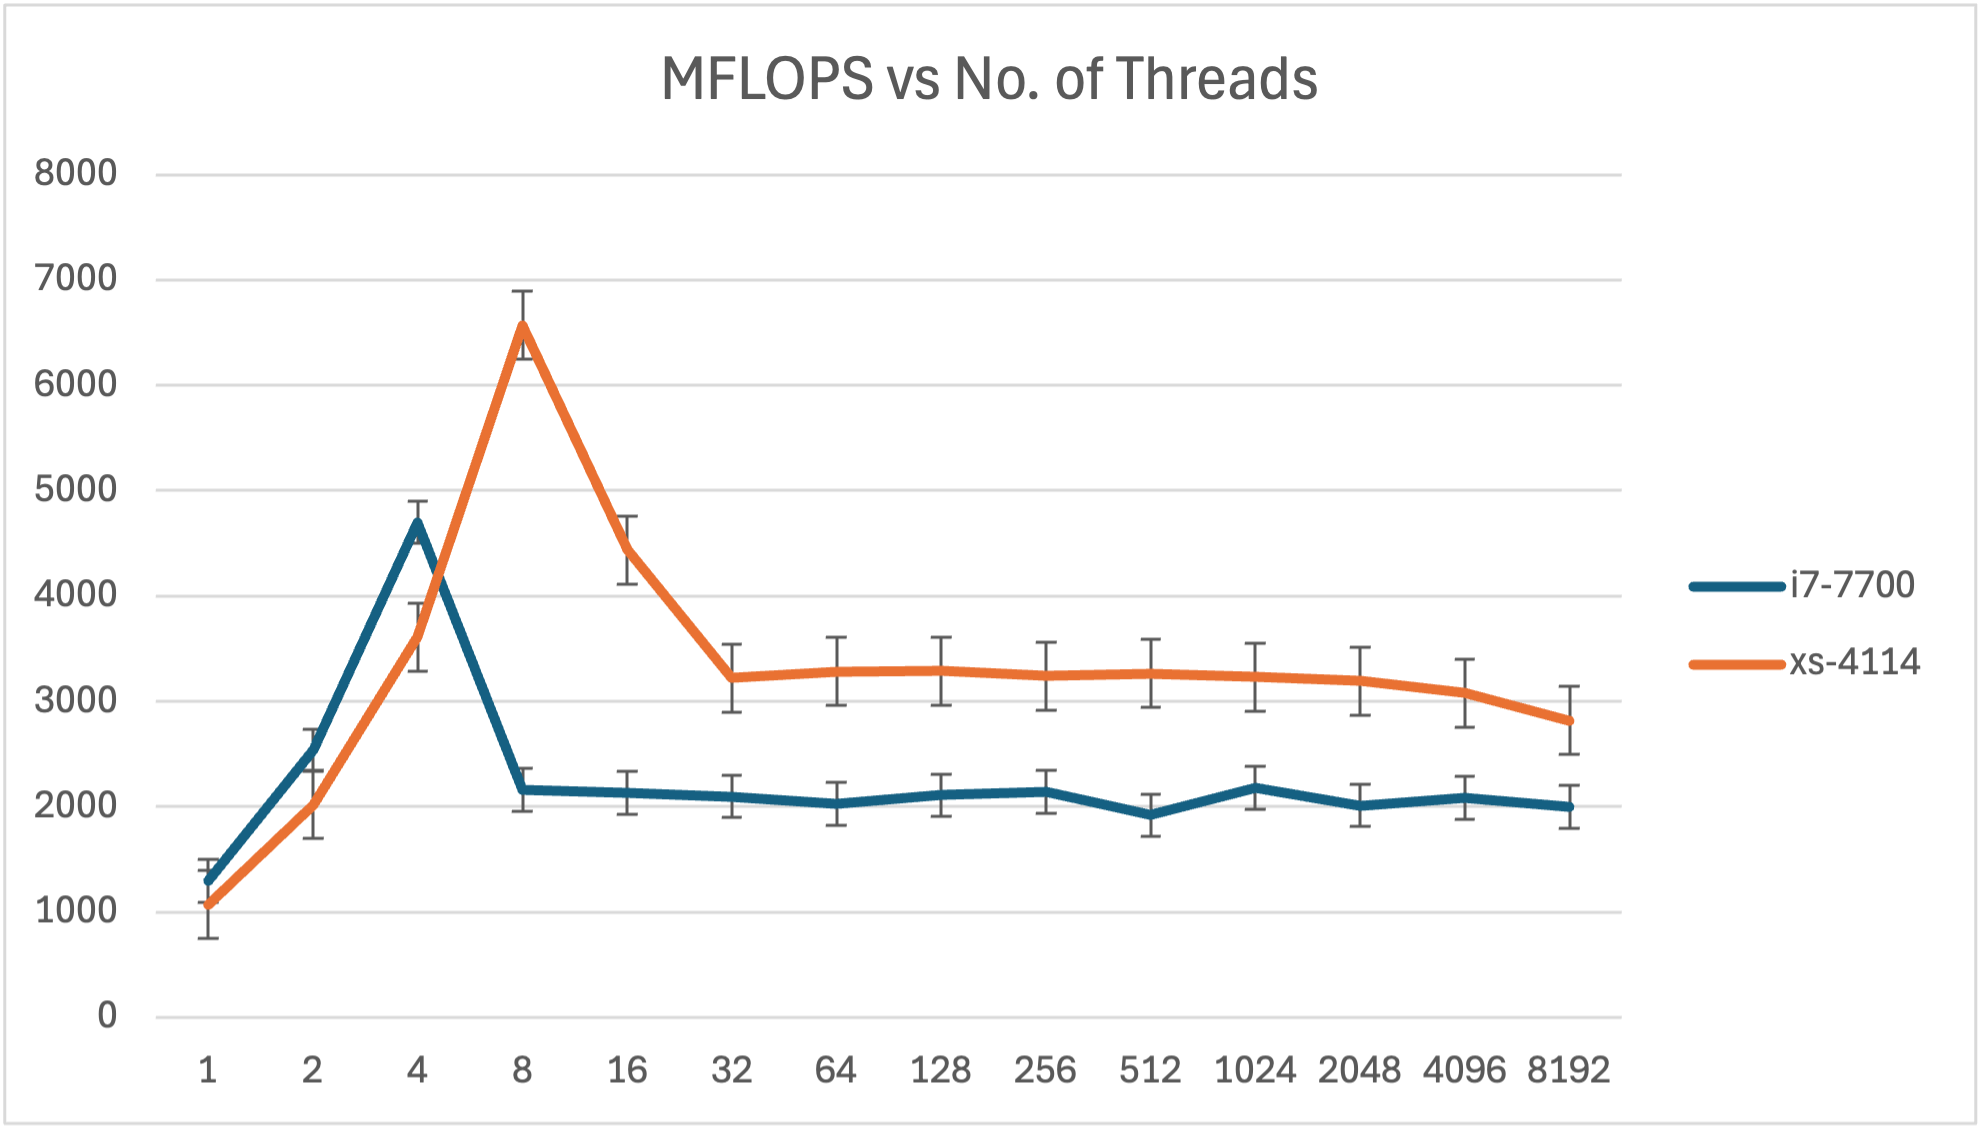
\includegraphics[width=0.8\textwidth]{mflops.png}
		\caption{MFLOPS vs. threads}
		\label{fig:mflopsGraph}
	\end{subfigure}
	\caption{Comparison of processor performance vs. threads (Logarithmic X-axis)}
	\label{fig:graphsColWise}
\end{figure}

According to Intel, the i7-7700 processor has 4 physical cores and 8 logical cores while the XS-4114 processor has 10 physical cores and 20 logical cores. From figure \ref{fig:graphsColWise}, we can see that as the number of threads vary from 1 to the number of physical cores each respective processor has, the execution time of the program decreases significantly, the number of floating point operations (FLOPS) increases significantly, while the number of instructions per cycle (IPC) stays relatively constant. After the number of threads exceeds the number of physical cores, the program execution time begins to increase, FLOPS decrease, and IPC drop drastically. At 4 threads and below, the performance of the i7-7700 edges out the XS-4114. Beyond 4 threads, the XS-4114 performs better with lower execution time and higher FLOPS.

With 2 threads and a matrix size of 1000, \texttt{perf stat -r 3} reported that the i7-7700 had a mean clock rate 4.077 GHz while the XS-4114 had a mean clock rate of 2.770 GHz over 3 repetitions, and both processors had a similar number of IPC. This explains the better performance of the i7-7700 below 4 threads. With 8 threads and a matrix size of 1000, \texttt{perf stat -r 3} reported that while the clock rate of the i7-7700 was still higher, the XS-4114 had a significantly higher mean IPC of 1.73 compared to 0.31, and significantly lower mean number of context switches at 9 compared to 311. This shows that the higher number of cores of the XS-4114 allows it to parallelize the higher number of threads far more effectively with a lower number of context switches. With 64 threads and a matrix size of 1000 on a XS-4114 node, \texttt{perf stat -r 3} reported a mean of 1,365 context switches and 0.32 IPC. This shows that a thread count beyond the number of physical cores results in a high context switch overhead which offsets any benefits gained from the increased number of threads.

\section{Column-wise vs Row-wise Multiplication}
In the multiplication of the 2 matrices $A \times B$, the elements in matrix $B$ were stored in row-major order and were accessed column-wise. A copy of the program was made and the copy was modified such that matrix B is stored in column-major order and the elements were accessed row-wise. The same tests performed previously were run on an XS-4114 processor node and the comparison with the previously obtained data is shown below.  

\begin{figure}[H]
	\centering
	\begin{subfigure}{0.5\textwidth}
		\centering
		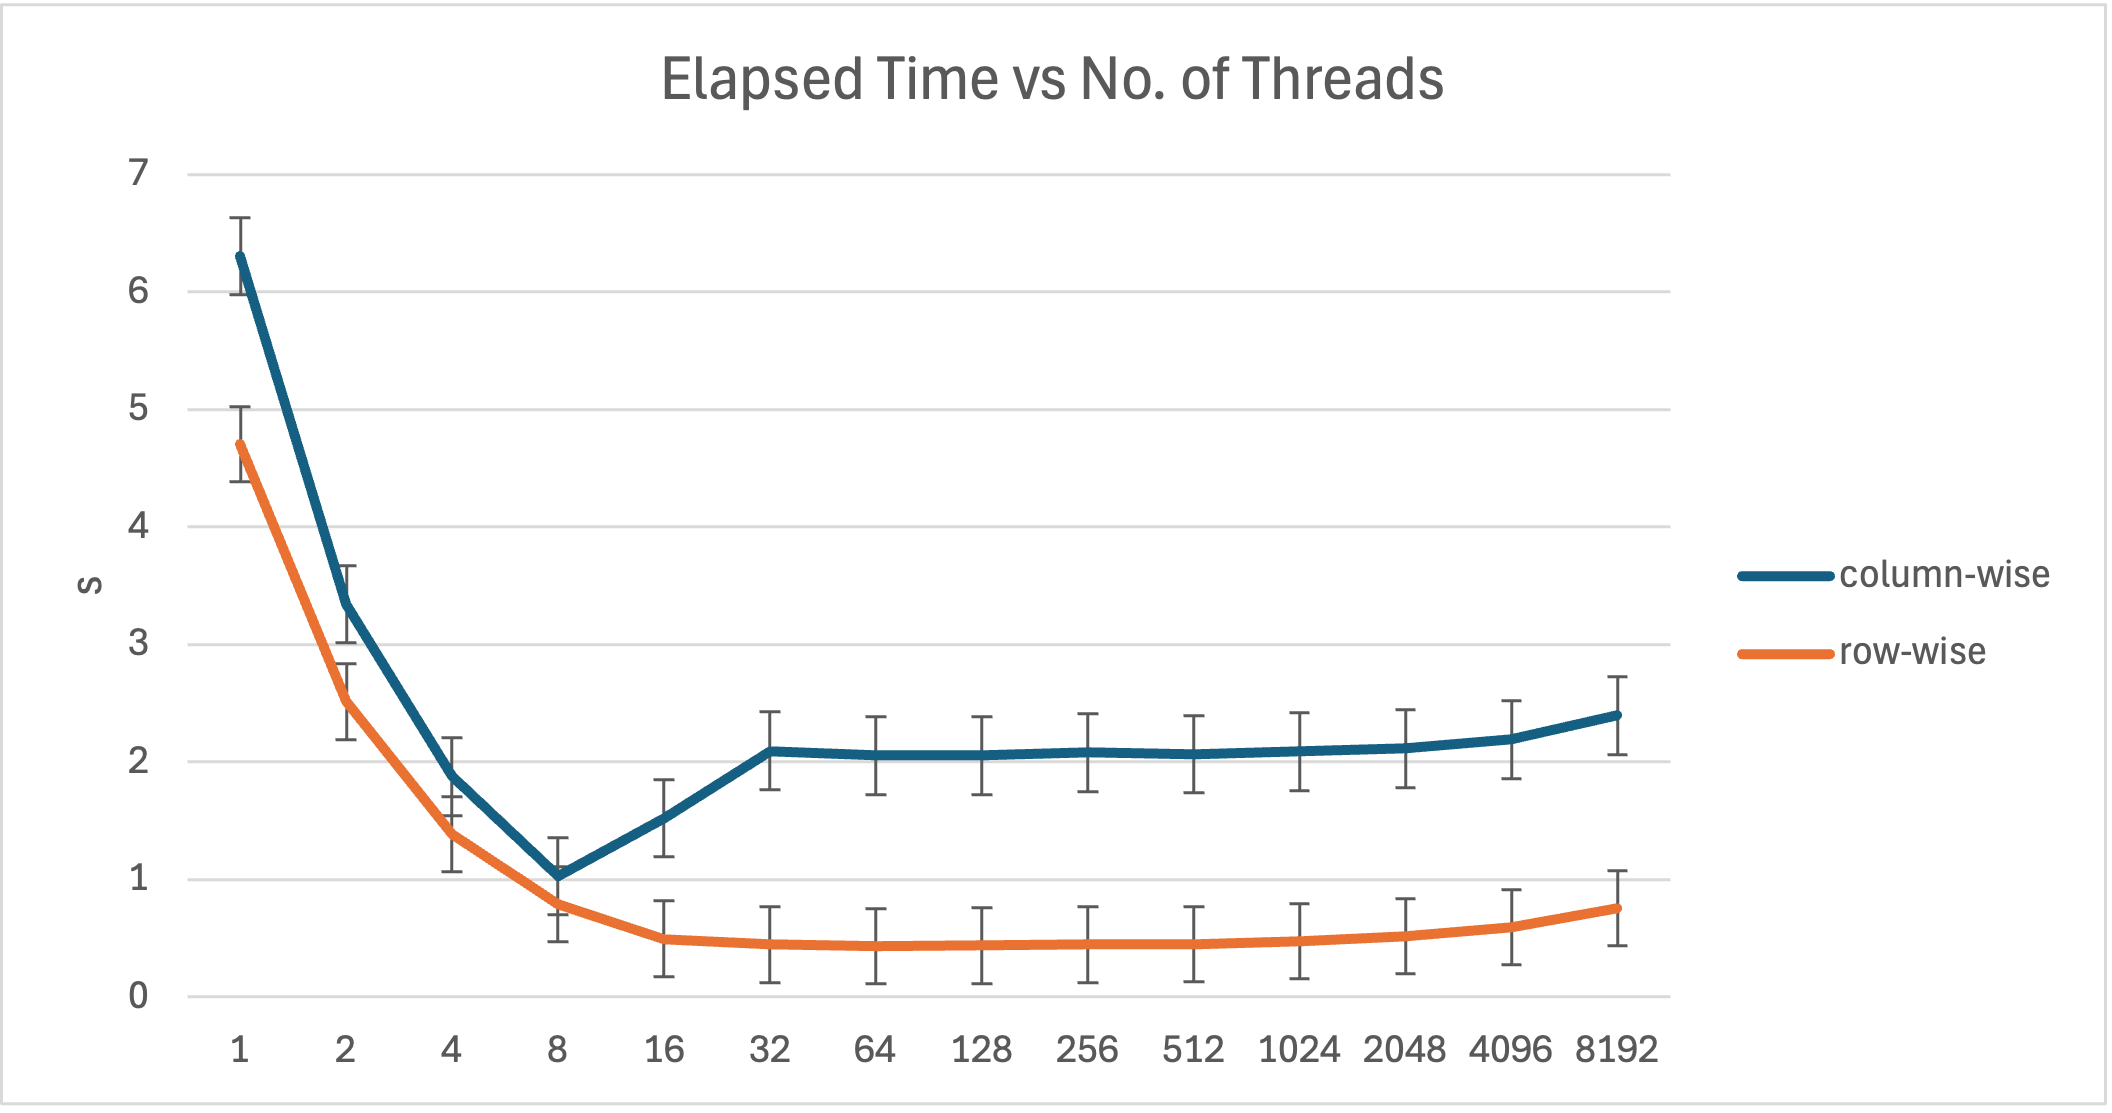
\includegraphics[width=0.8\linewidth]{timeElapsedRowWise.png}
		\subcaption{Graph of time elapsed against number of threads}
		\label{fig:timeGraphRowWise}
	\end{subfigure}%
	\begin{subfigure}{0.5\textwidth}
		\centering
		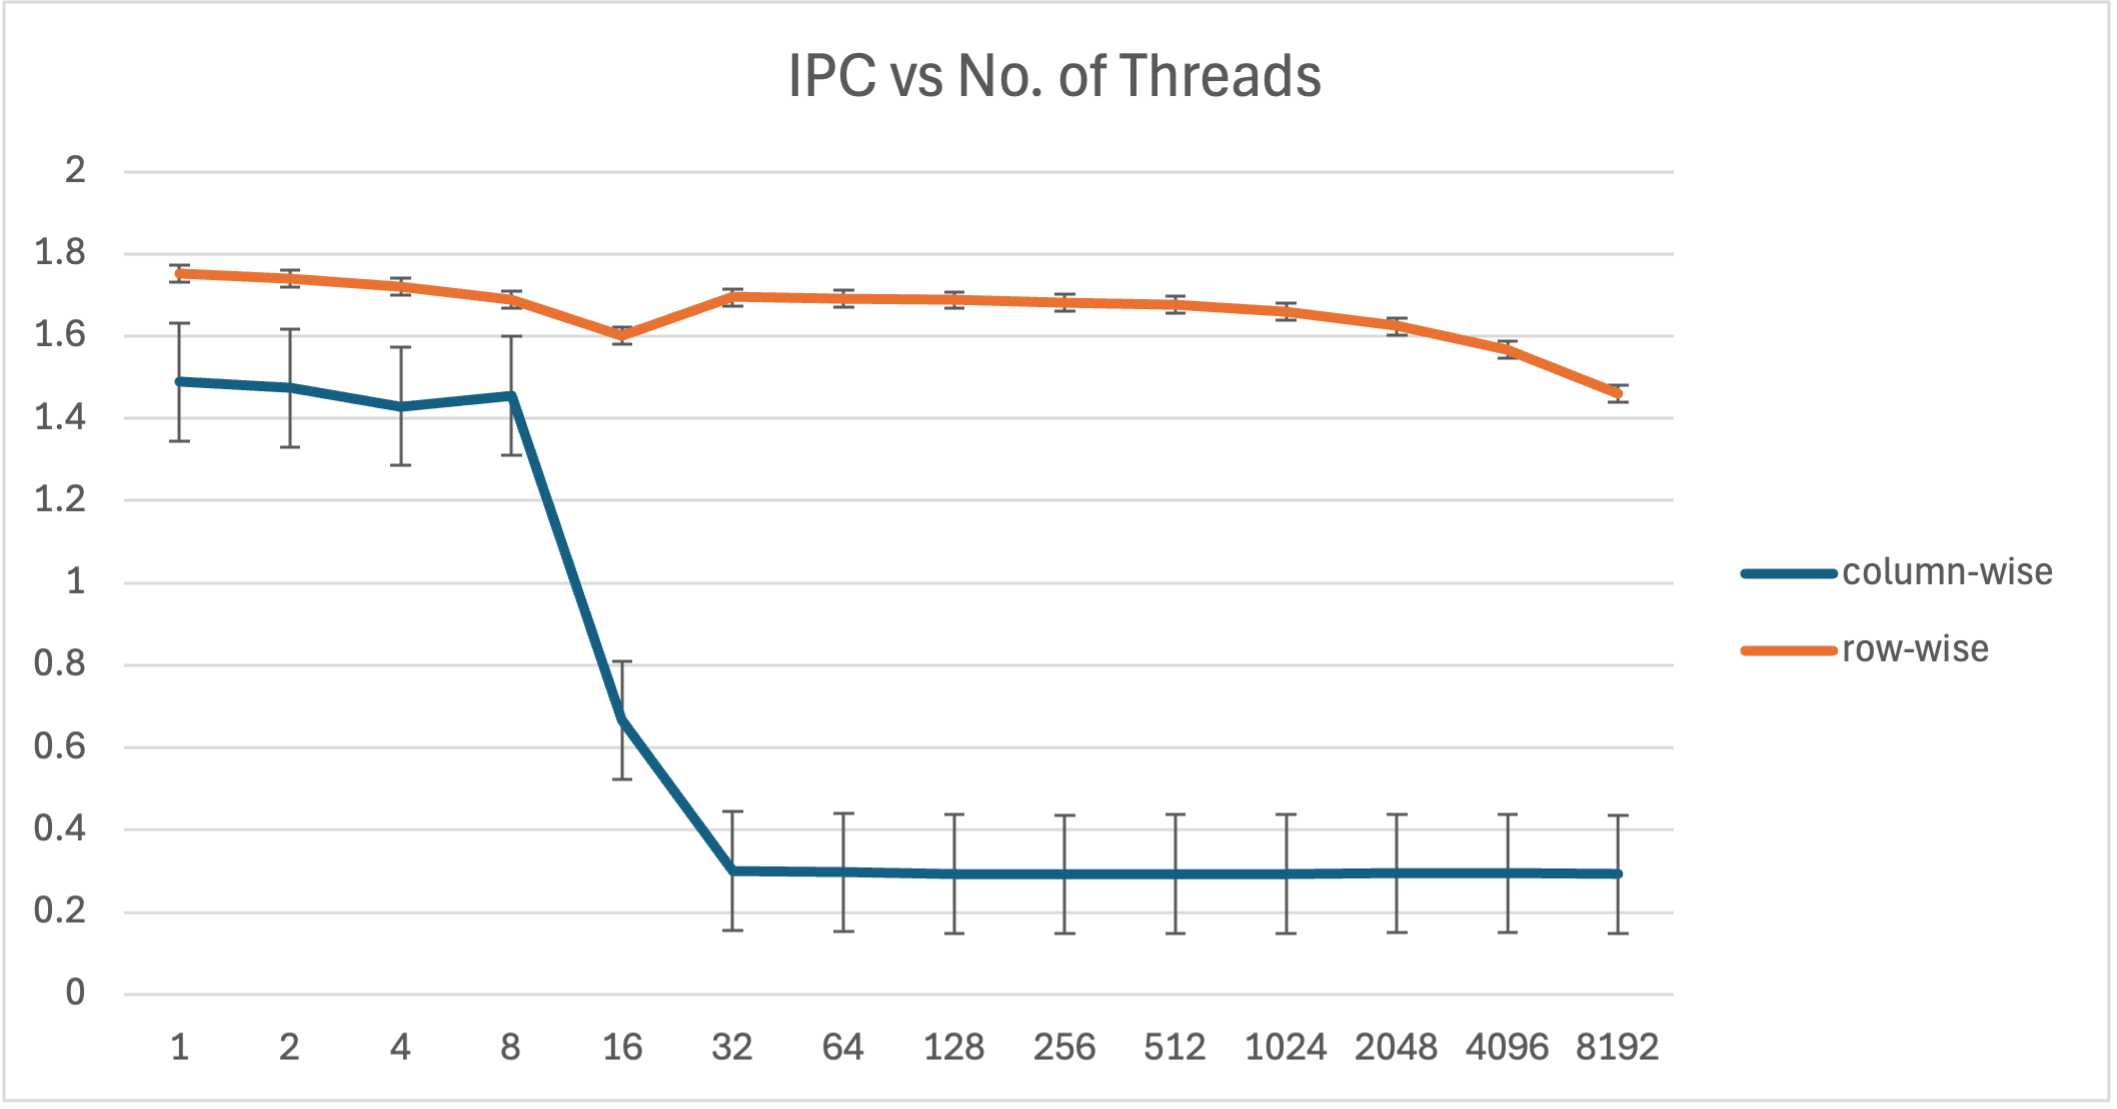
\includegraphics[width=0.8\linewidth]{ipcRowWise.png}
		\subcaption{Graph of Instructions per Cycle (IPC) against number of threads}
		\label{fig:ipcGraphRowWise}
	\end{subfigure}%
	\newline
	\begin{subfigure}{0.5\textwidth}
		\centering
		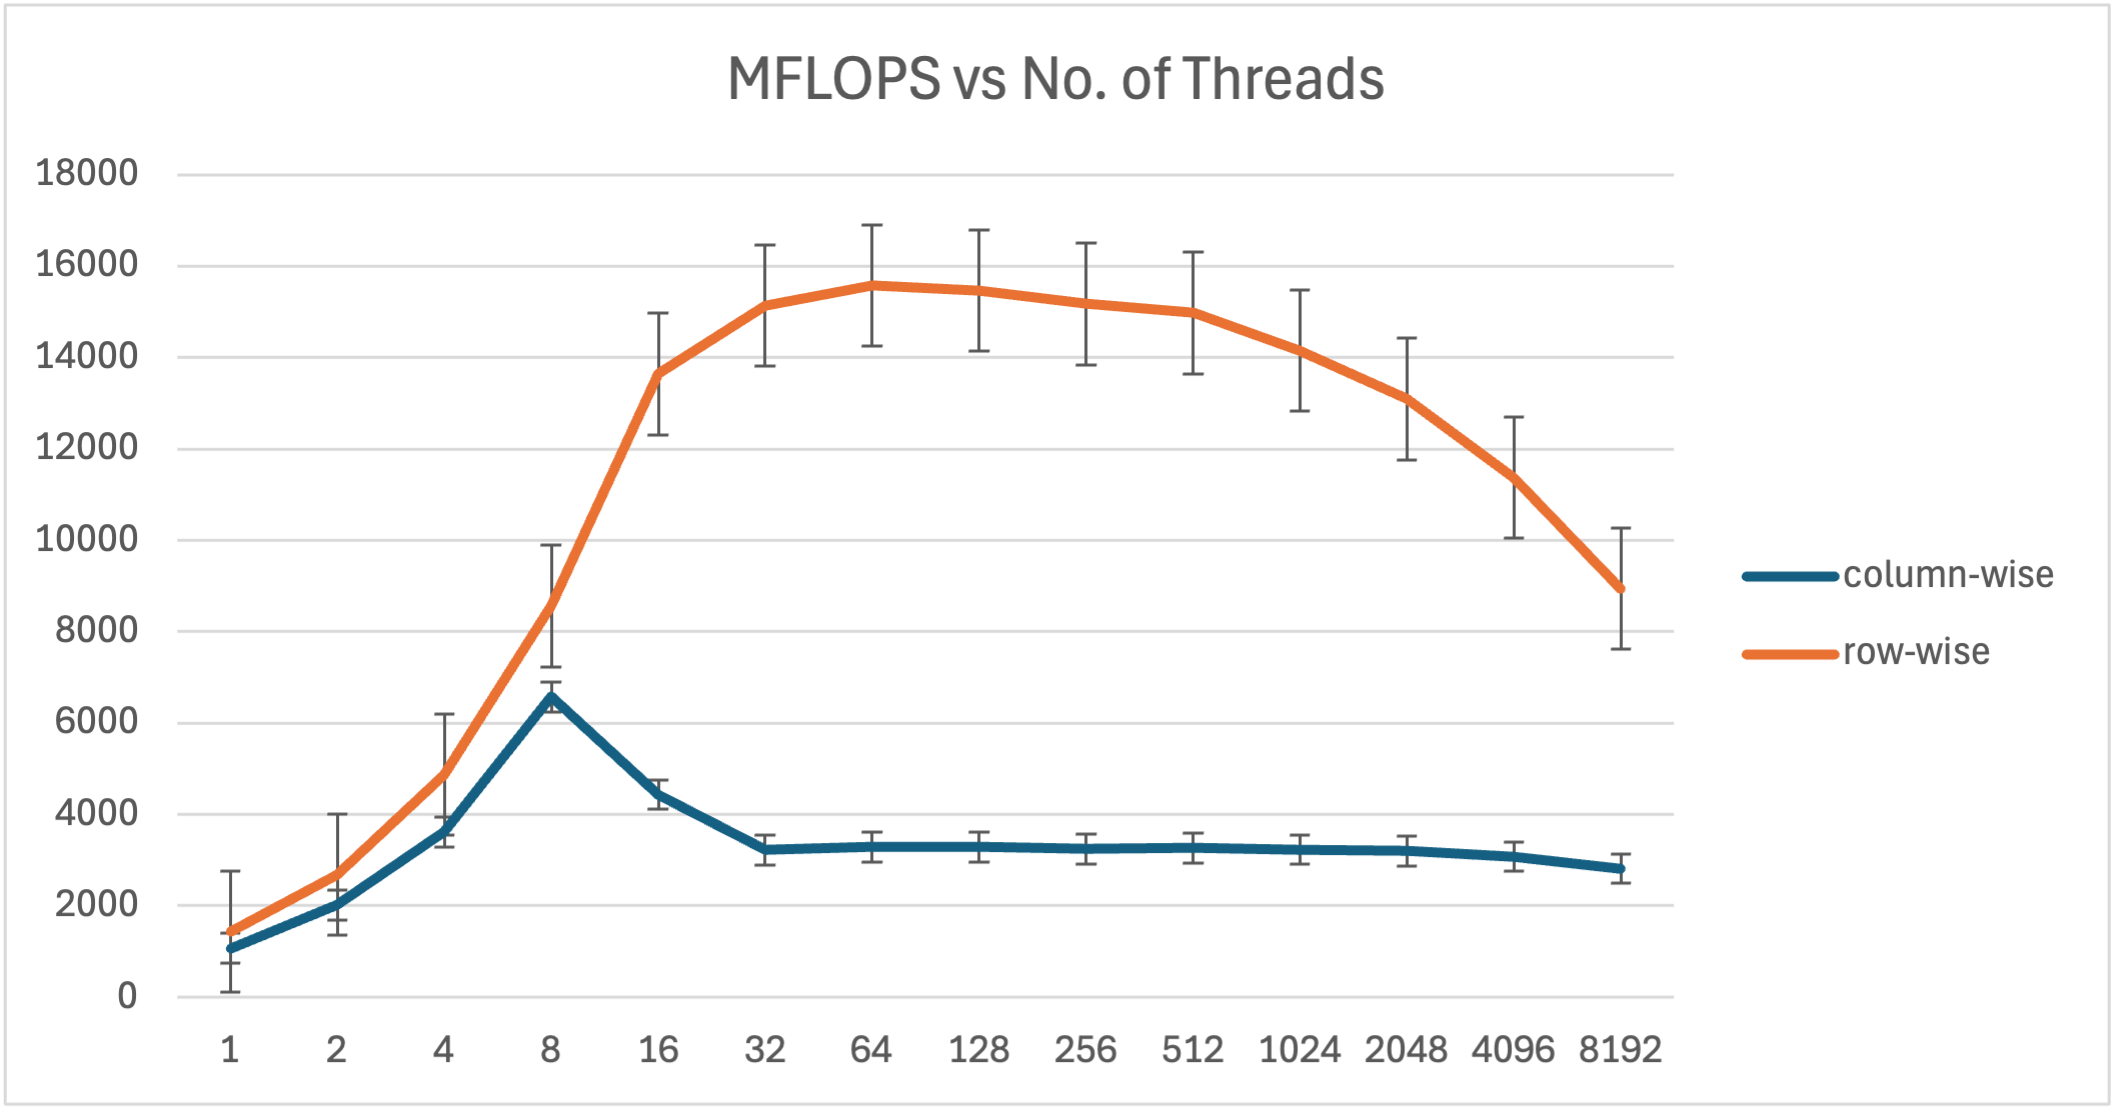
\includegraphics[width=0.8\textwidth]{mflopsRowWise.png}
		\caption{Graph of Millions of Floating Point Operations (MFLOPS) against number of threads}
		\label{fig:mflopsGraphRowWise}
	\end{subfigure}
	\caption{Graphs comparing column-wise and row-wise performance variation with number of threads (Logarithmic X-axis)}
	\label{fig:graphsRowWise}
\end{figure}

From figure \ref{fig:graphsRowWise}, we can see that performance significantly improves with row wise access during multiplication, especially at thread counts greater than the number of physical cores. With 2 threads, a matrix size of 1000, and execution on the XS-4114 processor, \texttt{perf stat -r 3 -e LLC-cache-loads,LLC-cache-misses,L1-dcache-loads,L1-dcache-load-misses} reports an L1-dcache miss rate of 39.19\% and 3.11\% for column-wise multiplication and row-wise multiplication respectively. This shows that row-wise multiplication has improved spatial locality, reducing the number of L1-cache misses, which could explain the improved performance of row-wise multiplication.

The measurements above were repeated, adding the \texttt{resource\_stalls.any} event. At 2 threads and a matrix size of 1000, both column-wise and row-wise multiplication had about 1.97 billion resource stalls. Increasing the number of threads to 16 resulted in 780 million and 12 billion resource stalls for row-wise and column-wise multiplication respectively. This explains the further increased performance of row-wise multiplication at higher thread counts.

\newpage

\begin{appendices}

\section{Reproduction}
Experiments used Slurm nodes \texttt{soctf-pdc-005} (XS-4114) and \texttt{soctf-pdf-013} (i7-7700). Code was compiled with \texttt{g++ 12.3.0} using flags \texttt{-O3 -fopenmp -g}. Execution was managed via \texttt{srun/sbatch}, with metrics collected using \texttt{perf 5.15.168}. Raw data, scripts, source code, and figures are available at \url{https://github.com/ginloy/CS3210-labs/tree/main/L2}. Script outputs are in .slurmlog files, raw data is in csv files, processed data is in the excel file, source code for column-wise and row-wise multiplication are in mm-omp.cpp and mm-omp-rows.cpp respectively.

\end{appendices}

\end{document}
